% ================= Section 3 =================
\clearpage
\section{資料庫概念設計 (Conceptual Design of the Database)}

\subsection{Entity Relationship (ER) Model}

圖 \ref{fig:er} 是 e-Shop 的 ER 圖，依 2.4 節的資料需求與 2.8 節的商業規則繪製，使用 Chen 記號，共有 9 個實體（其中 ORDER\_ITEM、STATUS\_HISTORY 為弱實體）與 13 個關係。圖的排列由左上往右下閱讀：最上面一列是使用者與商品，中間是折扣與商店，再往下是訂單與訂單明細，最下面是訂單狀態歷程與退貨申請。關係名稱也都可以由上往下、由左往右讀成一句話，例如「USER PLACES ORDER」、「ORDER CONTAINS ORDER\_ITEM」。


圖中使用的記號如表 \ref{tab:notation}。

\begin{xltabular}{\linewidth}{|>{\centering\arraybackslash}p{4.2cm}|>{\raggedright\arraybackslash}X|}
\caption{ER 圖記號}\label{tab:notation}\\
\hline\rowcolor{headgray}\textbf{記號} & \textbf{意義}\\\hline\endfirsthead
\hline\rowcolor{headgray}\textbf{記號} & \textbf{意義}\\\hline\endhead
矩形 & 實體（entity）\\\hline
雙線矩形 & 弱實體（weak entity）\\\hline
菱形 & 關係（relationship）\\\hline
雙線菱形 & 識別關係（identifying relationship），連接弱實體與其擁有者\\\hline
橢圓 & 屬性\\\hline
屬性名稱加底線 & 鍵屬性（key attribute）\\\hline
屬性名稱加虛線底線 & 弱實體的部分鍵（partial key）\\\hline
雙線橢圓 & 多值屬性（multivalued attribute）\\\hline
虛線橢圓 & 衍生屬性（derived attribute），不另外儲存，查詢時計算\\\hline
橢圓再連出橢圓 & 複合屬性（composite attribute）\\\hline
雙線連線 & 全部參與（total participation）\\\hline
單線連線 & 部分參與（partial participation）\\\hline
1、N、M & 基數比（cardinality ratio）\\\hline
\end{xltabular}

\begin{landscape}
\begin{figure}[p]
\centering
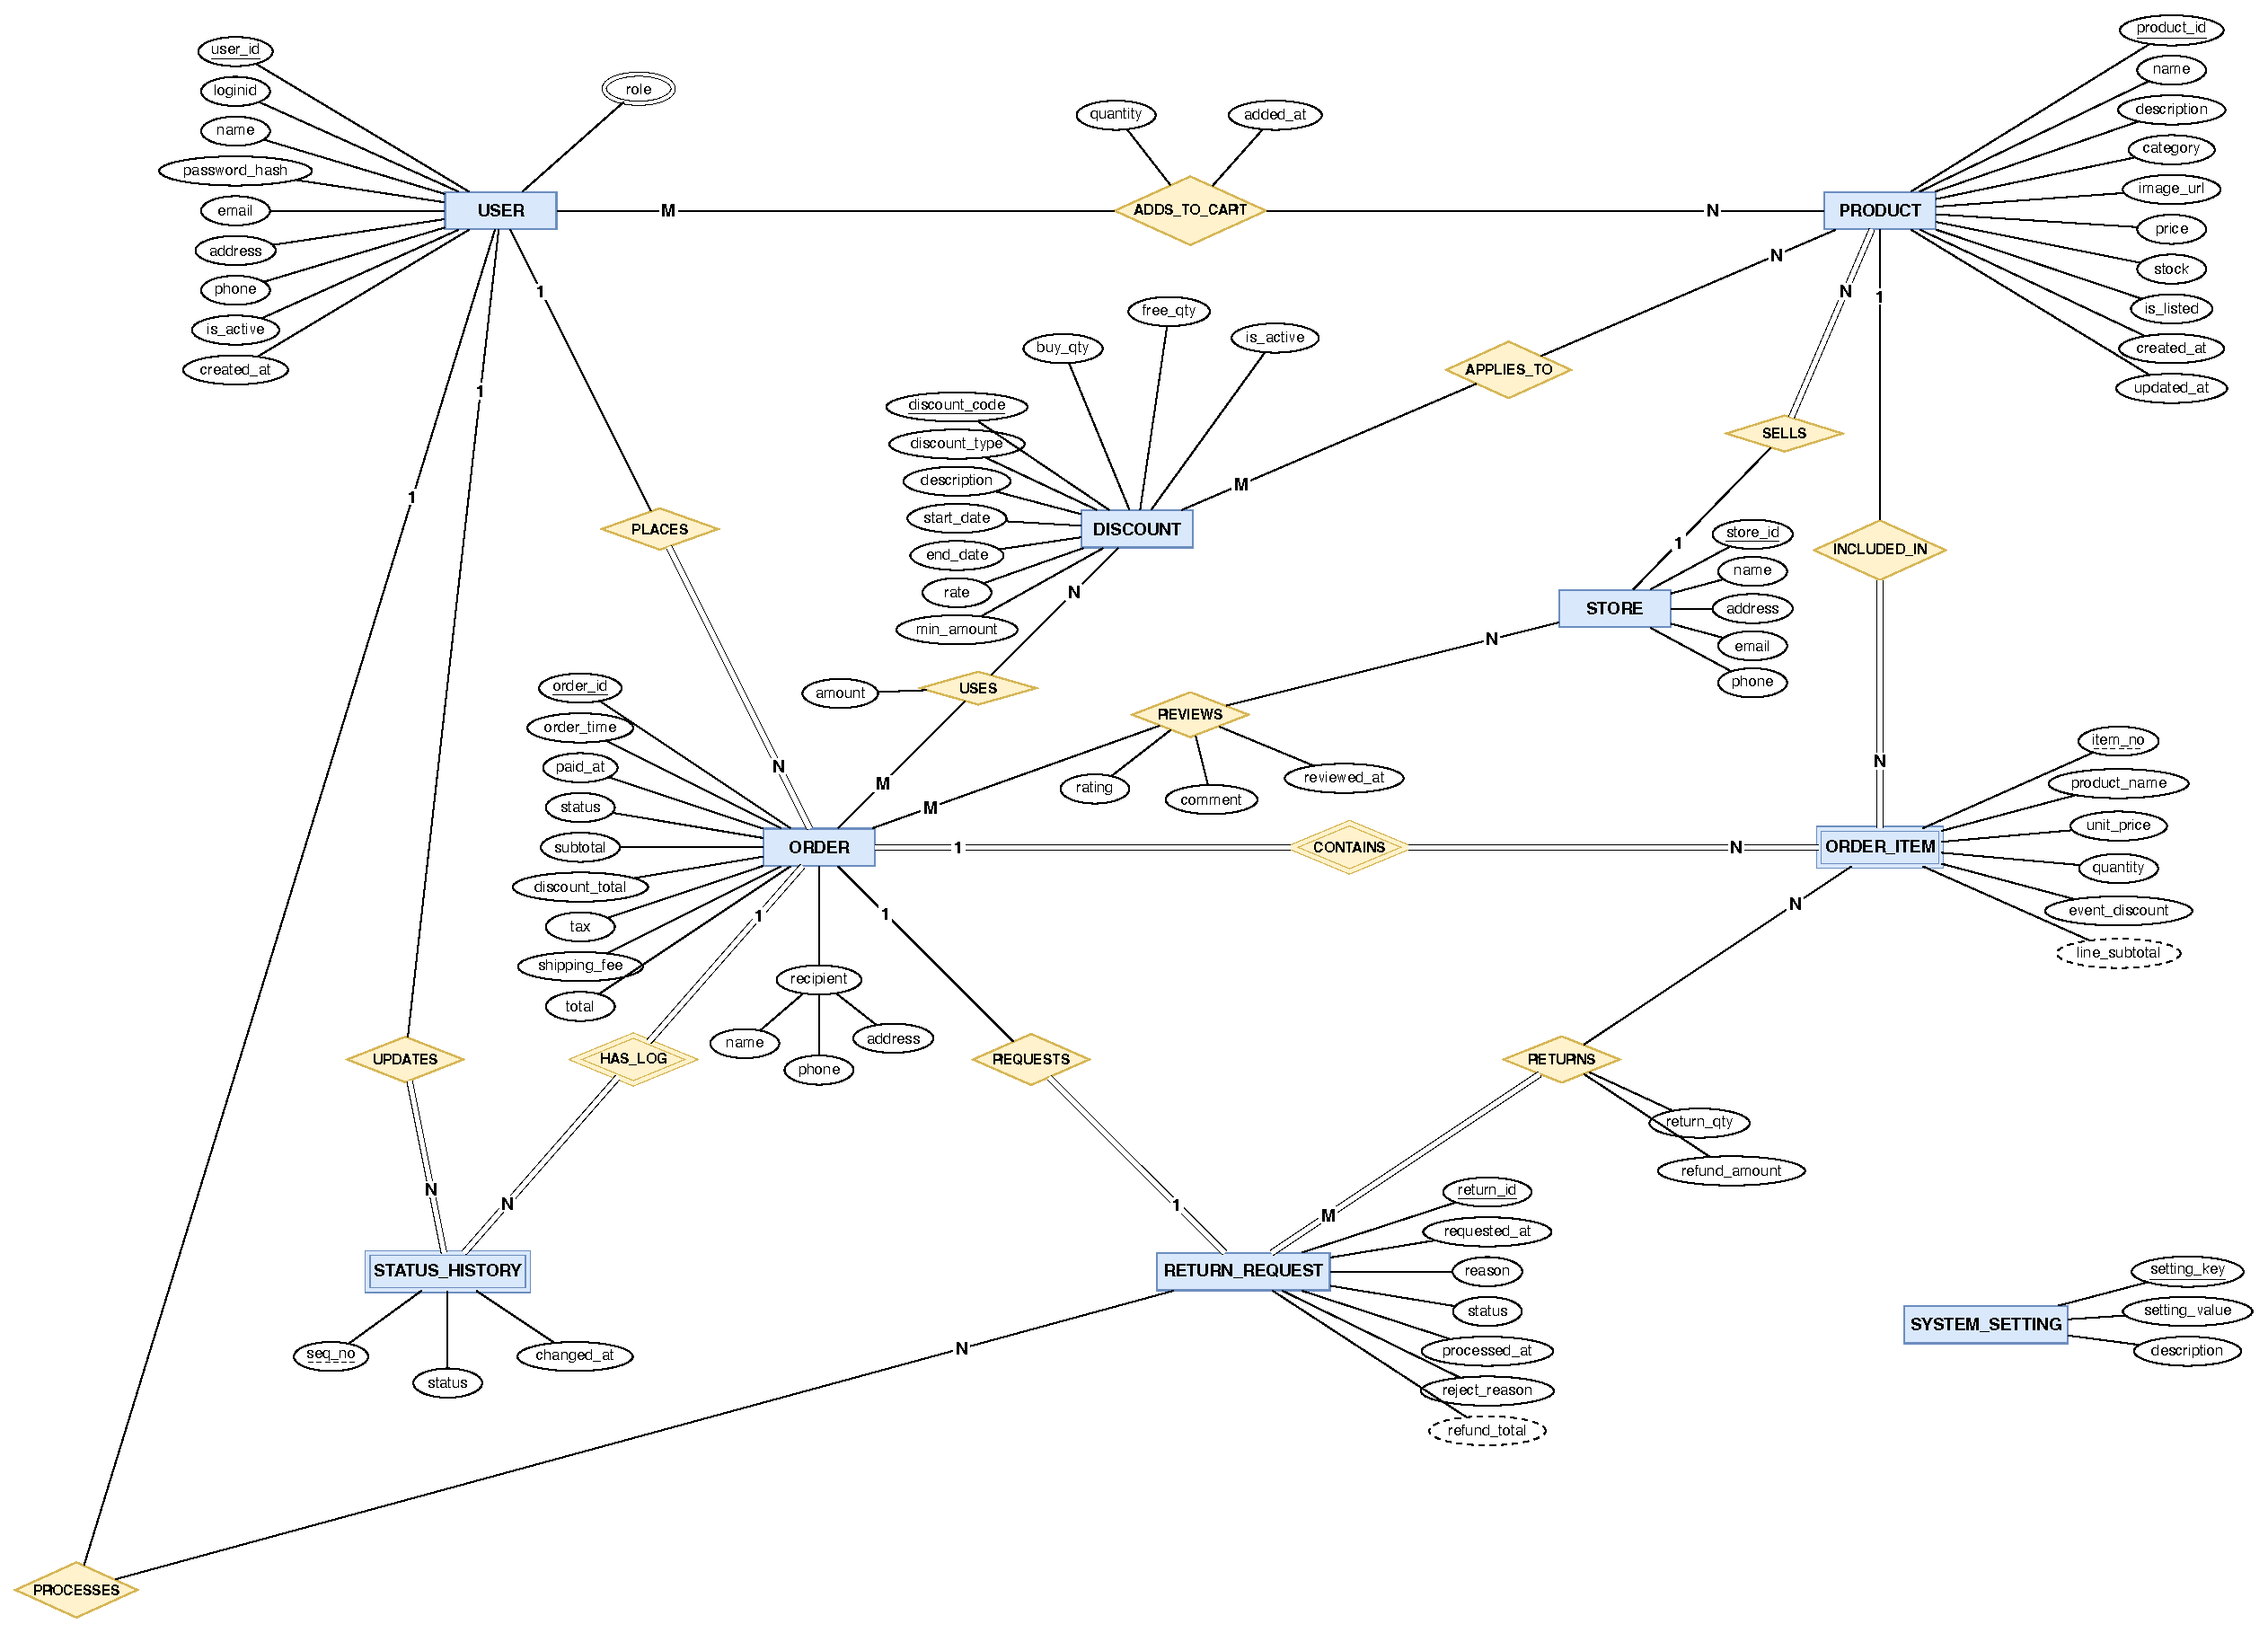
\includegraphics[width=\linewidth,height=0.93\textheight,keepaspectratio]{ER圖/ER_drawio.pdf}
\caption{e-Shop ER Diagram}\label{fig:er}
\end{figure}
\end{landscape}

\subsection{實體說明 (Entities)}

表 \ref{tab:entity} 說明每個實體存放的資料、鍵與屬性。各屬性的資料型態、是否可為 NULL 與限制，列在 4.2 節。

\begingroup\small
\begin{xltabular}{\linewidth}{|>{\raggedright\arraybackslash}p{3.1cm}|>{\raggedright\arraybackslash}X|>{\raggedright\arraybackslash}p{3.2cm}|>{\raggedright\arraybackslash}p{3.6cm}|}
\caption{實體、鍵與屬性}\label{tab:entity}\\
\hline\rowcolor{headgray}\textbf{實體} & \textbf{說明} & \textbf{鍵} & \textbf{屬性}\\\hline\endfirsthead
\hline\rowcolor{headgray}\textbf{實體} & \textbf{說明} & \textbf{鍵} & \textbf{屬性}\\\hline\endhead
USER & 系統所有使用者（顧客、工作人員、系統管理員）。loginid 由使用者自己取，所以另外以系統產生的 user\_id 當主鍵；一位使用者可以有多個角色，所以 role 為多值屬性。 & 主鍵 \at{user_id}；候選鍵 \at{loginid} & loginid、name、password\_hash、email、address、phone、is\_active、created\_at、role（多值）\\\hline
PRODUCT & 商店販售的商品。已被訂單引用的商品不能刪除，只能把 is\_listed 改成 false 下架。 & 主鍵 \at{product_id} & name、description、category、image\_url、price、stock、is\_listed、created\_at、updated\_at\\\hline
DISCOUNT & 折扣政策。三種折扣共用一個實體，以 discount\_type 區分；用不到的規則參數為 NULL。 & 主鍵 \at{discount_code} & discount\_type、description、start\_date、end\_date、rate、min\_amount、buy\_qty、free\_qty、is\_active\\\hline
STORE & 販售商品的商店。 & 主鍵 \at{store_id} & name、address、email、phone\\\hline
ORDER & 顧客確認付款後成立的訂單。金額欄位是付款當下的計算結果，之後折扣或稅率改變也不能變動，所以儲存下來。 & 主鍵 \at{order_id} & order\_time、paid\_at、status、subtotal、discount\_total、tax、shipping\_fee、total、recipient（複合：name、phone、address）\\\hline
ORDER\_ITEM（弱實體） & 訂單中的每一項商品，保存下單當下的品名與單價（BR-08）。離開訂單就沒有意義，所以是 ORDER 的弱實體。 & 部分鍵 \at{item_no}；以 (\at{order_id}, \at{item_no}) 識別 & product\_name、unit\_price、quantity、event\_discount、line\_subtotal（衍生 = unit\_price × quantity）\\\hline
STATUS\_HISTORY（弱實體） & 訂單每一次狀態變更的紀錄（OMS-F-007、OMS-F-008）。 & 部分鍵 \at{seq_no}；以 (\at{order_id}, \at{seq_no}) 識別 & status、changed\_at\\\hline
RETURN\_REQUEST & 顧客提出的退貨申請。 & 主鍵 \at{return_id} & requested\_at、reason、status、processed\_at、reject\_reason、refund\_total（衍生 = 各退貨明細退款金額總和）\\\hline
SYSTEM\_SETTING & 稅率、基本運費等系統參數（BR-22），計算訂單金額時讀取，不和其他實體發生關係。 & 主鍵 \at{setting_key} & setting\_value、description\\\hline
\end{xltabular}
\endgroup

\subsection{關係、基數與參與限制 (Relationships)}

表 \ref{tab:rel} 依 ER 圖由上往下、由左往右的順序列出每個關係。「全部參與」表示該實體的每一筆資料都一定參與這個關係，在 ER 圖中以雙線表示。

\begingroup\small
\begin{xltabular}{\linewidth}{|>{\centering\arraybackslash}p{2.5cm}|>{\centering\arraybackslash}p{3.5cm}|>{\raggedright\arraybackslash}p{3.3cm}|>{\raggedright\arraybackslash}X|}
\caption{關係、基數與參與限制}\label{tab:rel}\\
\hline\rowcolor{headgray}\textbf{關係} & \textbf{實體與基數} & \textbf{參與限制} & \textbf{說明}\\\hline\endfirsthead
\hline\rowcolor{headgray}\textbf{關係} & \textbf{實體與基數} & \textbf{參與限制} & \textbf{說明}\\\hline\endhead
ADDS\_TO\_CART & USER M : N PRODUCT & 兩邊皆部分參與 & 顧客的購物車。關係屬性 quantity（大於 0）、added\_at；同一顧客的同一商品只有一筆（DR-04）。\\\hline
PLACES & USER 1 : N ORDER & ORDER 全部；USER 部分 & 每筆訂單屬於且僅屬於一位顧客（BR-07）；顧客可以沒有訂單，工作人員與管理員也不會下單。\\\hline
APPLIES\_TO & DISCOUNT M : N PRODUCT & 兩邊皆部分參與 & 特殊活動折扣適用的商品。只有 special\_event 類型的折扣會參與，同一商品的期間不得重疊（BR-13）。\\\hline
SELLS & STORE 1 : N PRODUCT & PRODUCT 全部；STORE 部分 & 每個商品屬於且僅屬於一間商店，一間商店可以販售零到多個商品（BR-03）。\\\hline
INCLUDED\_IN & PRODUCT 1 : N ORDER\_ITEM & ORDER\_ITEM 全部；PRODUCT 部分 & 每筆明細對應一個商品，報表依此統計各商品與商店的銷售；商品可以從未被購買。\\\hline
USES & ORDER M : N DISCOUNT & 兩邊皆部分參與 & 訂單實際套用的折扣，關係屬性 amount 為該折扣的折抵金額。三種折扣可同時套用（BR-11）。\\\hline
REVIEWS（選配） & ORDER M : N STORE & 兩邊皆部分參與 & 顧客對已完成訂單中買過的商店評分，關係屬性 rating（1～5）、comment、reviewed\_at；每筆訂單對每間商店最多評一次（BR-24）。\\\hline
CONTAINS（識別關係） & ORDER 1 : N ORDER\_ITEM & 兩邊皆全部參與 & 每筆訂單至少一項明細（BR-07），每筆明細一定屬於一筆訂單；同一訂單中同一商品只有一筆明細。\\\hline
HAS\_LOG（識別關係） & ORDER 1 : N STATUS\_HISTORY & 兩邊皆全部參與 & 訂單成立時就寫入第一筆 received 紀錄，所以每筆訂單至少有一筆歷程。\\\hline
UPDATES & USER 1 : N STATUS\_HISTORY & STATUS\_HISTORY 全部；USER 部分 & 每次狀態變更都記錄操作者：received、cancelled 由顧客觸發，其餘由工作人員更新。\\\hline
REQUESTS & ORDER 1 : 1 RETURN\_REQUEST & RETURN\_REQUEST 全部；ORDER 部分 & 每筆訂單最多只能申請一次退貨（BR-25），所以是 1 : 1。\\\hline
RETURNS & RETURN\_REQUEST M : N ORDER\_ITEM & RETURN\_REQUEST 全部；ORDER\_ITEM 部分 & 退貨申請要退的明細，可以只退部分商品。關係屬性 return\_qty（大於 0 且不超過購買數量）、refund\_amount（核准後依 BR-26 計算）。\\\hline
PROCESSES & USER 1 : N RETURN\_REQUEST & 兩邊皆部分參與 & 處理退貨申請的工作人員；pending 的申請還沒有處理者，所以 RETURN\_REQUEST 是部分參與。\\\hline
\end{xltabular}
\endgroup

\subsection{設計說明}

畫 ER 圖時有幾個地方可以有不同畫法，我們的選擇與理由如下：

\begin{enumerate}
  \item \textbf{角色用多值屬性。}題目說管理員也可以是工作人員，USER 只放一個 role 欄位表示不出來。也可以把顧客、工作人員、管理員畫成三個子類別，但三者的屬性完全一樣，只差在權限，所以用多值屬性 role，轉成資料表就是 \at{user_role}。
  \item \textbf{訂單明細是弱實體。}明細也可以畫成 ORDER 和 PRODUCT 之間的 M:N 關係，但退貨申請要指向「某筆訂單的某一項明細」，關係不能再和其他實體發生關係，所以畫成弱實體 ORDER\_ITEM。
  \item \textbf{特殊活動折扣的期間。}期間屬於 DISCOUNT，但 BR-13 要求同一商品的期間不能重疊，商品和期間要在同一張表才能用資料庫限制檢查，所以轉成資料表時 \at{product_discount} 會複製一份期間，並用複合外鍵確保和 \at{discount} 一致（見 4.3 節）。
  \item \textbf{商店評價連到 ORDER。}BR-24 要求顧客有已完成、且買過該店商品的訂單才能評價，每筆訂單對每間商店只能評一次。畫成 ORDER 和 STORE 的關係，主鍵就是（訂單, 商店），評論者就是訂單的顧客，不用另外存。
  \item \textbf{衍生屬性。}明細小計與退款總額可以直接算出，不另外儲存；訂單的金額欄位雖然也算得出來，但它們是付款當下的結果，必須保留，所以仍然儲存。
\end{enumerate}

\subsection{ER 圖無法表示的限制}

以下規則畫不進 ER 圖，4.3 節說明在資料庫中如何實作：

\begin{itemize}
  \item 只有具有 customer 角色的使用者能參與 PLACES 與 ADDS\_TO\_CART；只有 staff 能參與 PROCESSES（BR-21）。
  \item 購買數量不得超過商品目前的庫存，庫存不得為負數（BR-06）。
  \item 只有 special\_event 類型的折扣能參與 APPLIES\_TO，且同一商品的期間不能重疊（BR-13）。
  \item 訂單狀態只能依 received → processing → shipping → closed 前進；cancelled 只能從 received 變過去（BR-19）。
  \item 退貨數量不得超過購買數量；只有 processing、shipping、closed 的訂單可以申請退貨（BR-25）。
\end{itemize}

% ================= Section 4 =================
\clearpage
\section{邏輯資料庫綱要 (Logic Database Schema)}

\subsection{Schema of the Database}

我們依 ER-to-Relational mapping 的步驟把 ER 圖轉成 15 張資料表：一般實體各成一張表（複合屬性 recipient 拆成三個欄位，衍生屬性不建欄位）；弱實體的主鍵為擁有者主鍵加部分鍵；1:1 的 REQUESTS 把外鍵放在全部參與的 \at{return_request} 並設為 UNIQUE；1:N 關係在 N 端加外鍵；M:N 關係與多值屬性 role 各自成表。因為 user 與 order 是 SQL 保留字，這兩張表命名為 \at{users} 與 \at{orders}。

圖 \ref{fig:schema} 為 schema 圖，箭頭由外鍵欄位指向被參照的主鍵欄位，底線為主鍵，標 (FK) 為外鍵；複合外鍵只從第一個欄位畫一條箭頭。

\begin{landscape}
\begin{figure}[p]
\centering
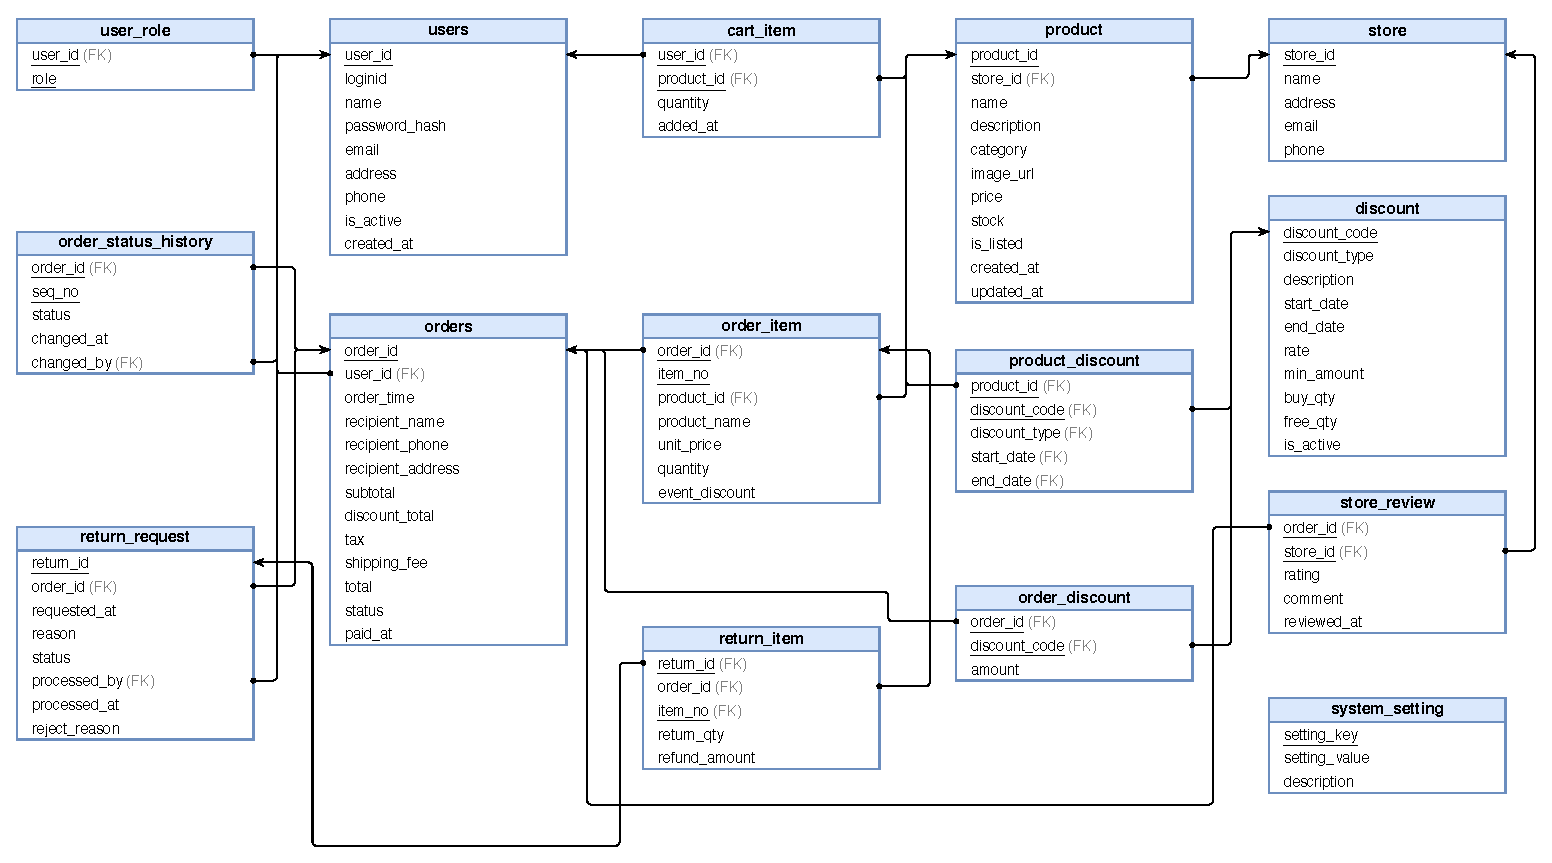
\includegraphics[width=\linewidth,height=0.9\textheight,keepaspectratio]{schema圖/schema_diagram.pdf}
\caption{e-Shop Schema Diagram}\label{fig:schema}
\end{figure}
\end{landscape}

\subsection{Domain of the Database}

以下列出每張資料表的欄位。金額一律以新台幣「元」為單位，用 \at{NUMERIC(10,0)} 存整數；折扣率用 \at{NUMERIC(4,3)}；編號類主鍵用 \at{SERIAL}（自動遞增整數）。Key 欄的 PK 為主鍵、FK 為外鍵。

\begin{domtable}{USERS}{存放所有使用者的帳號資料}
\dr{user_id}{SERIAL}{PK}{Not null}{使用者編號}
\dr{loginid}{VARCHAR(30)}{Unique}{Not null}{登入帳號，不可重複（BR-01）}
\dr{name}{VARCHAR(50)}{}{Not null}{姓名}
\dr{password_hash}{VARCHAR(100)}{}{Not null}{bcrypt 雜湊後的密碼}
\dr{email}{VARCHAR(100)}{}{Not null}{電子郵件}
\dr{address}{VARCHAR(200)}{}{}{地址}
\dr{phone}{VARCHAR(20)}{}{}{電話}
\dr{is_active}{BOOLEAN}{}{Not null}{帳號是否啟用，預設 TRUE}
\dr{created_at}{TIMESTAMP}{}{Not null}{建立時間，預設 now()}
\end{domtable}

\begin{domtable}{USER\_ROLE}{存放使用者的角色，一位使用者可以有多個角色}
\dr{user_id}{INT}{PK, FK}{Not null}{使用者編號 Reference (USERS)，ON DELETE CASCADE}
\dr{role}{VARCHAR(10)}{PK}{Not null}{角色，只能是 customer、staff、admin}
\end{domtable}

\begin{domtable}{STORE}{存放商店資料}
\dr{store_id}{SERIAL}{PK}{Not null}{商店編號}
\dr{name}{VARCHAR(50)}{}{Not null}{商店名稱}
\dr{address}{VARCHAR(200)}{}{Not null}{商店地址}
\dr{email}{VARCHAR(100)}{}{Not null}{聯絡 Email}
\dr{phone}{VARCHAR(20)}{}{Not null}{聯絡電話}
\end{domtable}

\begin{domtable}{PRODUCT}{存放商品資料}
\dr{product_id}{SERIAL}{PK}{Not null}{商品編號}
\dr{store_id}{INT}{FK}{Not null}{所屬商店 Reference (STORE)}
\dr{name}{VARCHAR(100)}{}{Not null}{商品名稱}
\dr{description}{TEXT}{}{}{商品描述}
\dr{category}{VARCHAR(30)}{}{}{分類}
\dr{image_url}{VARCHAR(300)}{}{}{商品圖片網址}
\dr{price}{NUMERIC(10,0)}{}{Not null}{售價（price > 0）}
\dr{stock}{INT}{}{Not null}{庫存數量（stock >= 0）}
\dr{is_listed}{BOOLEAN}{}{Not null}{是否上架，預設 TRUE}
\dr{created_at}{TIMESTAMP}{}{Not null}{上架時間}
\dr{updated_at}{TIMESTAMP}{}{Not null}{最後修改時間}
\end{domtable}

\begin{domtable}{CART\_ITEM}{存放顧客購物車中的商品}
\dr{user_id}{INT}{PK, FK}{Not null}{顧客編號 Reference (USERS)，ON DELETE CASCADE}
\dr{product_id}{INT}{PK, FK}{Not null}{商品編號 Reference (PRODUCT)，ON DELETE CASCADE}
\dr{quantity}{INT}{}{Not null}{數量（quantity > 0）}
\dr{added_at}{TIMESTAMP}{}{Not null}{加入時間}
\end{domtable}

\begin{domtable}{ORDERS}{存放訂單資料}
\dr{order_id}{SERIAL}{PK}{Not null}{訂單編號}
\dr{user_id}{INT}{FK}{Not null}{下單顧客 Reference (USERS)}
\dr{order_time}{TIMESTAMP}{}{Not null}{下單時間}
\dr{recipient_name}{VARCHAR(50)}{}{Not null}{收件人姓名}
\dr{recipient_phone}{VARCHAR(20)}{}{Not null}{收件人電話}
\dr{recipient_address}{VARCHAR(200)}{}{Not null}{收件地址}
\dr{subtotal}{NUMERIC(10,0)}{}{Not null}{商品小計（>= 0）}
\dr{discount_total}{NUMERIC(10,0)}{}{Not null}{折扣總額（>= 0），預設 0}
\dr{tax}{NUMERIC(10,0)}{}{Not null}{稅額（>= 0）}
\dr{shipping_fee}{NUMERIC(10,0)}{}{Not null}{運費（>= 0）}
\dr{total}{NUMERIC(10,0)}{}{Not null}{訂單總額（>= 0），計算方式見 BR-09、BR-10}
\dr{status}{VARCHAR(10)}{}{Not null}{訂單狀態：received、processing、shipping、closed、cancelled、returned，預設 received}
\dr{paid_at}{TIMESTAMP}{}{Not null}{確認付款時間}
\end{domtable}

\begin{domtable}{ORDER\_ITEM}{存放訂單明細；(order\_id, product\_id) 為 UNIQUE}
\dr{order_id}{INT}{PK, FK}{Not null}{訂單編號 Reference (ORDERS)，ON DELETE CASCADE}
\dr{item_no}{SMALLINT}{PK}{Not null}{明細序號（> 0）}
\dr{product_id}{INT}{FK}{Not null}{商品編號 Reference (PRODUCT)}
\dr{product_name}{VARCHAR(100)}{}{Not null}{下單當下的品名}
\dr{unit_price}{NUMERIC(10,0)}{}{Not null}{下單當下的單價（> 0）}
\dr{quantity}{INT}{}{Not null}{購買數量（> 0）}
\dr{event_discount}{NUMERIC(10,0)}{}{Not null}{特殊活動折抵金額，介於 0 與 unit\_price × quantity 之間，預設 0}
\end{domtable}

\begin{domtable}{ORDER\_STATUS\_HISTORY}{存放訂單狀態變更紀錄}
\dr{order_id}{INT}{PK, FK}{Not null}{訂單編號 Reference (ORDERS)，ON DELETE CASCADE}
\dr{seq_no}{SMALLINT}{PK}{Not null}{變更序號（> 0）}
\dr{status}{VARCHAR(10)}{}{Not null}{變更後的狀態（同 ORDERS.status 的六種）}
\dr{changed_at}{TIMESTAMP}{}{Not null}{變更時間}
\dr{changed_by}{INT}{FK}{Not null}{操作者 Reference (USERS)}
\end{domtable}

\begin{domtable}{DISCOUNT}{存放折扣政策；另有表格層級 CHECK 依類型限制規則參數（BR-17）}
\dr{discount_code}{VARCHAR(20)}{PK}{Not null}{折扣代碼，由系統產生}
\dr{discount_type}{VARCHAR(15)}{}{Not null}{shipping、seasonal、special\_event}
\dr{description}{VARCHAR(200)}{}{Not null}{折扣說明}
\dr{start_date}{DATE}{}{Not null}{開始日期（start\_date <= end\_date）}
\dr{end_date}{DATE}{}{Not null}{結束日期}
\dr{rate}{NUMERIC(4,3)}{}{}{折扣率（0 < rate < 1）}
\dr{min_amount}{NUMERIC(10,0)}{}{}{運費折扣門檻（> 0）}
\dr{buy_qty}{SMALLINT}{}{}{買 X 送 Y 的 X（> 0）}
\dr{free_qty}{SMALLINT}{}{}{買 X 送 Y 的 Y（> 0），與 buy\_qty 同時有值或同時為 NULL}
\dr{is_active}{BOOLEAN}{}{Not null}{是否啟用，預設 TRUE}
\end{domtable}
表格層級 CHECK 的內容：shipping 只能有 min\_amount；seasonal 只能有 rate；special\_event 必須在 rate 與 buy\_qty／free\_qty 之中剛好選一種。另外 (discount\_code, discount\_type, start\_date, end\_date) 設為 UNIQUE，給 PRODUCT\_DISCOUNT 的複合外鍵使用。

\begin{domtable}{PRODUCT\_DISCOUNT}{存放特殊活動折扣適用的商品}
\dr{product_id}{INT}{PK, FK}{Not null}{商品編號 Reference (PRODUCT)，ON DELETE CASCADE}
\dr{discount_code}{VARCHAR(20)}{PK, FK}{Not null}{折扣代碼}
\dr{discount_type}{VARCHAR(15)}{FK}{Not null}{只能是 special\_event}
\dr{start_date}{DATE}{FK}{Not null}{折扣開始日期}
\dr{end_date}{DATE}{FK}{Not null}{折扣結束日期}
\end{domtable}
(discount\_code, discount\_type, start\_date, end\_date) 為複合外鍵 Reference (DISCOUNT)，ON UPDATE CASCADE、ON DELETE CASCADE；並有 EXCLUDE 限制防止同一商品的期間重疊（見 4.3 節）。

\begin{domtable}{ORDER\_DISCOUNT}{存放訂單實際套用的折扣}
\dr{order_id}{INT}{PK, FK}{Not null}{訂單編號 Reference (ORDERS)，ON DELETE CASCADE}
\dr{discount_code}{VARCHAR(20)}{PK, FK}{Not null}{折扣代碼 Reference (DISCOUNT)}
\dr{amount}{NUMERIC(10,0)}{}{Not null}{該折扣的折抵金額（>= 0）}
\end{domtable}

\begin{domtable}{RETURN\_REQUEST}{存放退貨申請；(return\_id, order\_id) 為 UNIQUE，給 RETURN\_ITEM 的複合外鍵使用}
\dr{return_id}{SERIAL}{PK}{Not null}{退貨申請編號}
\dr{order_id}{INT}{FK, Unique}{Not null}{訂單編號 Reference (ORDERS)；每筆訂單只能申請一次}
\dr{requested_at}{TIMESTAMP}{}{Not null}{申請時間}
\dr{reason}{VARCHAR(300)}{}{Not null}{退貨原因}
\dr{status}{VARCHAR(10)}{}{Not null}{pending、approved、rejected，預設 pending}
\dr{processed_by}{INT}{FK}{}{處理的工作人員 Reference (USERS)；pending 時為 NULL}
\dr{processed_at}{TIMESTAMP}{}{}{處理時間；pending 時為 NULL}
\dr{reject_reason}{VARCHAR(300)}{}{}{拒絕原因；只有 rejected 時必須填寫}
\end{domtable}

\begin{domtable}{RETURN\_ITEM}{存放退貨申請要退的明細}
\dr{return_id}{INT}{PK, FK}{Not null}{退貨申請編號；(return\_id, order\_id) Reference (RETURN\_REQUEST)}
\dr{order_id}{INT}{FK}{Not null}{訂單編號；確保退的明細屬於同一筆訂單}
\dr{item_no}{SMALLINT}{PK, FK}{Not null}{明細序號；(order\_id, item\_no) Reference (ORDER\_ITEM)}
\dr{return_qty}{INT}{}{Not null}{退貨數量（> 0）}
\dr{refund_amount}{NUMERIC(10,0)}{}{}{該項退款金額（>= 0），核准前為 NULL}
\end{domtable}

\begin{domtable}{STORE\_REVIEW}{存放商店評價（選配）}
\dr{order_id}{INT}{PK, FK}{Not null}{訂單編號 Reference (ORDERS)}
\dr{store_id}{INT}{PK, FK}{Not null}{商店編號 Reference (STORE)}
\dr{rating}{SMALLINT}{}{Not null}{評分（1 至 5）}
\dr{comment}{VARCHAR(500)}{}{}{評論內容}
\dr{reviewed_at}{TIMESTAMP}{}{Not null}{評價時間}
\end{domtable}

\begin{domtable}{SYSTEM\_SETTING}{存放系統參數，例如 tax\_rate = 0.05、base\_shipping\_fee = 100}
\dr{setting_key}{VARCHAR(30)}{PK}{Not null}{參數名稱}
\dr{setting_value}{VARCHAR(50)}{}{Not null}{參數值}
\dr{description}{VARCHAR(100)}{}{}{參數說明}
\end{domtable}

\subsection{完整性限制的實作}

\textbf{參考完整性。}外鍵預設為 NO ACTION，被參照的資料不能直接刪除。例如商品已出現在訂單明細中就刪不掉，只能把 is\_listed 改成 false；用過的折扣與有訂單的顧客也一樣，符合 BR-20。只有「跟著主體一起消失也沒關係」的資料設定 ON DELETE CASCADE，例如使用者的角色與購物車、商品的購物車項目與折扣設定、訂單的明細與狀態歷程。

\textbf{特殊活動折扣期間不重疊（BR-13）。}做法分三步：(1) \at{product_discount} 存一份期間，用複合外鍵參照 \at{discount}，期間一定和折扣政策相同，修改折扣期間時 ON UPDATE CASCADE 會自動同步；(2) \at{discount_type} 以 CHECK 限定為 special\_event，運費與季節性折扣掛不到商品上；(3) 使用 PostgreSQL 的 EXCLUDE 限制，讓同一個 product\_id 的兩筆資料期間（含首尾兩日）不能有交集：
\begin{Verbatim}[fontsize=\small,xleftmargin=2em]
EXCLUDE USING gist (product_id WITH =,
                    daterange(start_date, end_date, '[]') WITH &&)
\end{Verbatim}

\textbf{以 CHECK 與 UNIQUE 處理的規則。}BR-01、BR-04、BR-05、BR-14、BR-15、BR-17、BR-19 的狀態值範圍、BR-24 的評分範圍與每單每店一則評價、BR-25 的每筆訂單只能申請一次退貨，都已寫在 4.2 節的欄位限制中。我們把 schema 寫成 SQL（Appendix）並在 PostgreSQL 上實際建立，用故意違規的資料測試（重複的 loginid、數量為 0、庫存扣成負數、期間重疊、不合法的狀態、同一訂單第二次申請退貨、退別張訂單的明細等），資料庫都會拒絕。

\textbf{需要在交易或 trigger 中處理的規則。}以下規則牽涉其他資料表或狀態的前後順序，預計在 Phase 3 以 trigger 或後端交易實作：

\begingroup\small
\begin{xltabular}{\linewidth}{|>{\centering\arraybackslash}p{1.6cm}|>{\raggedright\arraybackslash}X|>{\raggedright\arraybackslash}p{5.2cm}|}
\caption{需要 trigger 或交易處理的規則}\\
\hline\rowcolor{headgray}\textbf{規則} & \textbf{內容} & \textbf{預計做法}\\\hline\endfirsthead
\hline\rowcolor{headgray}\textbf{規則} & \textbf{內容} & \textbf{預計做法}\\\hline\endhead
BR-06 & 購買數量不得超過庫存 & 結帳交易中以 SELECT … FOR UPDATE 鎖定商品再扣庫存；stock >= 0 的 CHECK 是最後一道防線\\\hline
BR-07 & 每筆訂單至少一項明細 & 結帳交易中一起寫入訂單與明細\\\hline
BR-19 & 狀態只能依序前進 & orders 的 BEFORE UPDATE trigger 比對新舊狀態，並自動寫入 order\_status\_history\\\hline
BR-21 & 只有顧客能下單、只有工作人員能處理退貨 & trigger 檢查 user\_role，後端 API 也會檢查\\\hline
BR-24 & 只能評價已完成且買過該店商品的訂單 & store\_review 的 BEFORE INSERT trigger\\\hline
BR-25 & 退貨數量不超過購買數量；只有特定狀態的訂單能申請 & return\_request、return\_item 的 BEFORE INSERT trigger\\\hline
\end{xltabular}
\endgroup
